%!TEX program = xelatex

\documentclass[11pt,titlepage]{report}
%!TEX root = main.tex

\usepackage[T1]{fontenc}
\usepackage{lmodern}
\usepackage[svgnames]{xcolor}
\usepackage{fontspec} % XeLaTeX required!
\usepackage{graphicx}
\usepackage{circuitikz}
\usepackage{tikz}
\usepackage{pifont}
\usepackage[some]{background}
\usepackage{xltxtra} 
\usepackage{setspace}
\usepackage[absolute]{textpos}
\usepackage[latin1]{inputenc}
\usepackage[english]{babel}
\usepackage{graphicx}
\usepackage{wrapfig}
\usepackage{fullpage}
\usepackage[margin=1in]{geometry}
\usepackage{float}
\usepackage{url}
\usepackage{multicol}
\usepackage{hyperref}
\usepackage{titlepic}
\usepackage{standalone}
\usepackage{siunitx}
\usepackage{booktabs}
\usepackage{amsmath}
\usepackage{unicode-math}
\usepackage{verbatim}
\usepackage{enumitem}
\usepackage{listings}
\usepackage{multirow}
\usepackage{pgfplots}
\pgfplotsset{compat=1.8}
\usepackage{caption} 
\usepackage[parfill]{parskip}
\usepackage{import}
\usepackage[backend=bibtexu,texencoding=utf8,bibencoding=utf8,style=ieee,sortlocale=en_GB,language=auto]{biblatex}
\usepackage[strict,autostyle]{csquotes}
\usepackage[final]{pdfpages}
\usepackage{subcaption}
\usepackage{ifplatform}
%\captionsetup[table]{skip=10pt}


% Fix for includepdf bug in Mac OS X
\newcommand{\insertpdfpath}[1]{
	\ifwindows
	\newcommand{\insertpdf}[2]{\includepdf[pages=##1]{##2}}
	\else
	\newcommand{\insertpdf}[2]{\includepdf[pages=##1]{#1/##2}}
	\fi
}

%set fonts
\setmainfont[Ligatures=TeX]{Myriad Pro}
\setmathfont{Asana Math}
\setmonofont{Lucida Console}

\usepackage{titlesec, color}
\renewcommand{\familydefault}{\sfdefault} %set font family
\renewcommand{\arraystretch}{1.2} %set table vertical spacing
\setlength\parindent{0pt} %no paragraph indent
\hypersetup{ %setup hyperlinks
    colorlinks,
    citecolor=black,
    filecolor=black,
    linkcolor=black,
    urlcolor=black
}

%redesign chapter headings
\definecolor{gray75}{gray}{0.75}
\newcommand{\chapternumber}{\thechapter}
\newcommand{\hsp}{\hspace{20pt}}
\titleformat{\chapter}[hang]{\Huge\bfseries}{\chapternumber\hsp\textcolor{gray75}{|}\hsp}{0pt}{\Huge\bfseries}

%Redefine appendix headers
\renewcommand{\appendixname}{Appendix}
\renewcommand{\appendixtocname}{Appendices}
\renewcommand{\appendixpagename}{Appendices}

%For code listings
\definecolor{black}{rgb}{0,0,0}
\definecolor{browntags}{rgb}{0.65,0.1,0.1}
\definecolor{bluestrings}{rgb}{0,0,1}
\definecolor{graycomments}{rgb}{0.4,0.4,0.4}
\definecolor{redkeywords}{rgb}{1,0,0}
\definecolor{bluekeywords}{rgb}{0.13,0.13,0.8}
\definecolor{greencomments}{rgb}{0,0.5,0}
\definecolor{redstrings}{rgb}{0.9,0,0}
\definecolor{purpleidentifiers}{rgb}{0.01,0,0.01}


\lstdefinestyle{csharp}{
language=[Sharp]C,
showspaces=false,
showtabs=false,
breaklines=true,
showstringspaces=false,
breakatwhitespace=true,
escapeinside={(*@}{@*)},
columns=fullflexible,
commentstyle=\color{greencomments},
keywordstyle=\color{bluekeywords}\bfseries,
stringstyle=\color{redstrings},
identifierstyle=\color{purpleidentifiers},
basicstyle=\ttfamily\small}

\lstdefinestyle{c}{
language=C,
showspaces=false,
showtabs=false,
breaklines=true,
showstringspaces=false,
breakatwhitespace=true,
escapeinside={(*@}{@*)},
columns=fullflexible,
commentstyle=\color{greencomments},
keywordstyle=\color{bluekeywords}\bfseries,
stringstyle=\color{redstrings},
identifierstyle=\color{purpleidentifiers},
}

\lstdefinestyle{matlab}{
language=Matlab,
showspaces=false,
showtabs=false,
breaklines=true,
showstringspaces=false,
breakatwhitespace=true,
escapeinside={(*@}{@*)},
columns=fullflexible,
commentstyle=\color{greencomments},
keywordstyle=\color{bluekeywords}\bfseries,
stringstyle=\color{redstrings},
identifierstyle=\color{purpleidentifiers}
}

\lstdefinestyle{vhdl}{
language=VHDL,
showspaces=false,
showtabs=false,
breaklines=true,
showstringspaces=false,
breakatwhitespace=true,
escapeinside={(*@}{@*)},
columns=fullflexible,
commentstyle=\color{greencomments},
keywordstyle=\color{bluekeywords}\bfseries,
stringstyle=\color{redstrings},
identifierstyle=\color{purpleidentifiers}
}

\lstdefinestyle{xaml}{
language=XML,
showspaces=false,
showtabs=false,
breaklines=true,
showstringspaces=false,
breakatwhitespace=true,
escapeinside={(*@}{@*)},
columns=fullflexible,
commentstyle=\color{greencomments},
keywordstyle=\color{redkeywords},
stringstyle=\color{bluestrings},
tagstyle=\color{browntags},
morestring=[b]",
  morecomment=[s]{<?}{?>},
  morekeywords={xmlns,version,typex:AsyncRecords,x:Arguments,x:Boolean,x:Byte,x:Char,x:Class,x:ClassAttributes,x:ClassModifier,x:Code,x:ConnectionId,x:Decimal,x:Double,x:FactoryMethod,x:FieldModifier,x:Int16,x:Int32,x:Int64,x:Key,x:Members,x:Name,x:Object,x:Property,x:Shared,x:Single,x:String,x:Subclass,x:SynchronousMode,x:TimeSpan,x:TypeArguments,x:Uid,x:Uri,x:XData,Grid.Column,Grid.ColumnSpan,Click,ClipToBounds,Content,DropDownOpened,FontSize,Foreground,Header,Height,HorizontalAlignment,HorizontalContentAlignment,IsCancel,IsDefault,IsEnabled,IsSelected,Margin,MinHeight,MinWidth,Padding,SnapsToDevicePixels,Target,TextWrapping,Title,VerticalAlignment,VerticalContentAlignment,Width,WindowStartupLocation,Binding,Mode,OneWay,xmlns:x}
}

\lstdefinestyle{matlab}{
language=Matlab,
showspaces=false,
showtabs=false,
breaklines=true,
showstringspaces=false,
breakatwhitespace=true,
escapeinside={(*@}{@*)},
columns=fullflexible,
commentstyle=\color{greencomments},
keywordstyle=\color{bluekeywords}\bfseries,
stringstyle=\color{purpleidentifiers},
identifierstyle=\color{purpleidentifiers}
}

%defaults
\lstset{
basicstyle=\ttfamily\small,
extendedchars=false,
numbers=left,
numberstyle=\ttfamily\tiny,
stepnumber=1,
tabsize=4,
numbersep=5pt
}
\addbibresource{../../library/bibliography.bib}

% Fancy comb dirac, can be ignored for now. For further use.
%
% \usepackage[OT2,T1]{fontenc}
% \newcommand{\sha}{\text{\fontencoding{OT2}\selectfont\char88}}
% \newcommand{\F}[1]{\operatorname{\mathcal{F}}\left\{#1\right\}}
% \begin{equation}
% 	\F{\operatorname{rect}(F_s t) \ast 2F_s \sha(2F_s t)}
% \end{equation}

\begin{document}

\section{Labday 2}
\subsection{Report 8}
In this report the suitability of four test signals are investigated. Figure \ref{fig:ass-1-rep-8} shows the autocorrelation of all four signals. We see that the autocorrelation functions of maximum phase and minimum phase are closely related. The autocorrelation functions of the sinusoidal and BPSK signal differ from the other functions.

\begin{figure}[H]
	\centering
	\begin{subfigure}{0.49\textwidth}
		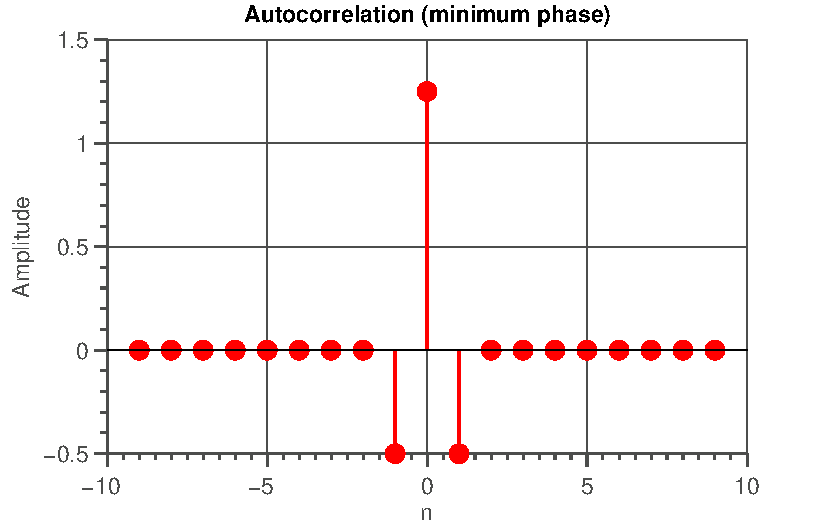
\includegraphics[width=\textwidth]{../../deliverable-7-resources/figures/ass-1/report-8-9-10/report-8/ass-1-report-8-minimum-phase-minimum-phase.pdf}
		\caption{Autocorrelation of a minimum phase signal}
	\end{subfigure}
	\begin{subfigure}{0.49\textwidth}
		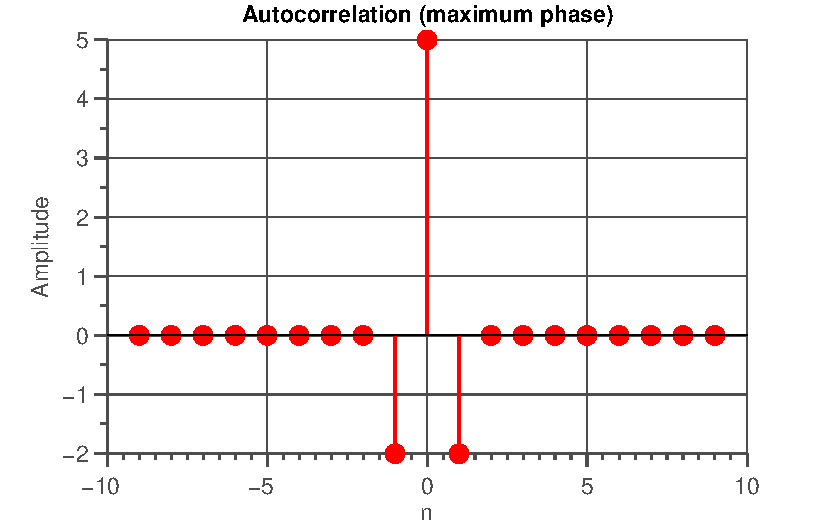
\includegraphics[width=\textwidth]{../../deliverable-7-resources/figures/ass-1/report-8-9-10/report-8/ass-1-report-8-maximum-phase-maximum-phase.pdf}
		\caption{Autocorrelation of a maximum phase signal}
	\end{subfigure}
	\begin{subfigure}{0.49\textwidth}
		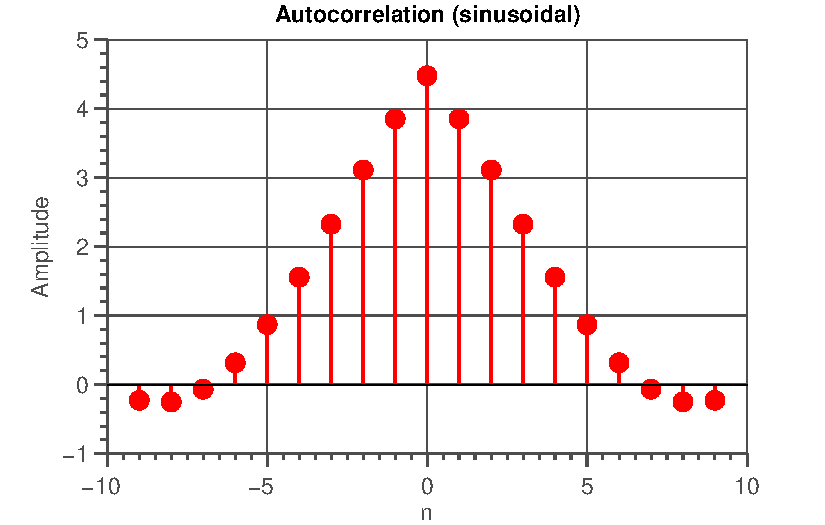
\includegraphics[width=\textwidth]{../../deliverable-7-resources/figures/ass-1/report-8-9-10/report-8/ass-1-report-8-sinusoidal-sinusoidal.pdf}
		\caption{Autocorrelation of a sinusoidal signal}
	\end{subfigure}
	\begin{subfigure}{0.49\textwidth}
		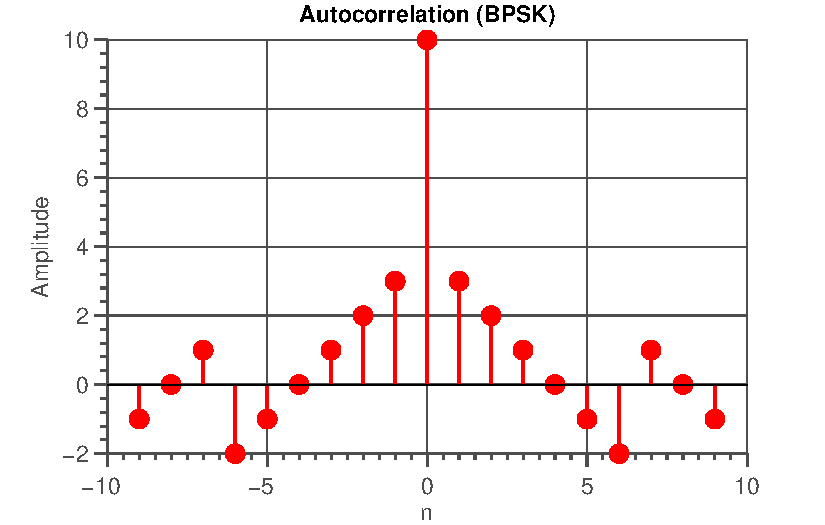
\includegraphics[width=\textwidth]{../../deliverable-7-resources/figures/ass-1/report-8-9-10/report-8/ass-1-report-8-BPSK-BPSK.pdf}
		\caption{Autocorrelation of a BPSK signal}
	\end{subfigure}
	\caption{Autocorrelation sequences of each of the tested signals}
	\label{fig:ass-1-rep-8}
\end{figure}

The Matched Filter yields a channel estimation $\hat{h}[n]$ given by
\[
	\hat{h}[n] = h[n] \ast r[n]
\]
where $h[n]$ denotes the channel impulse response and $r[n]$ the training sequence's autocorrelation function. If we require that $\hat{h}[n] \rightarrow h[n]$, then obviously $r[n] \rightarrow \delta[n]$. Therefore, we require $r[n]$ to only have a peak at $n=0$. This makes the minimum phase of maximum phase signal the most suitable test signal. However, both have side lobes of $1/2.5$ the peak's height, so they are not optimal. Note that for signals of greater length, the BPSK's autocorrelation is expected to be superior.
 
\subsection{Report 9}
Let $\hat{L}$ denote the lenght of the estimated channel impulse response $\hat{\vec{h}}$ and $L$ the length of the actual channel impulse response $\vec{h}$. Figure~\ref{fig:ass-1-rep-9-no-noise} shows the corrected channel estimation error $||\hat{\vec{h}}(\hat{\vec{h}} \cdot \vec{h})/(\hat{\vec{h}} \cdot \hat{\vec{h}}) - \vec{h}||$.
\begin{figure}[H]
	\centering
	\begin{subfigure}{0.49\textwidth}
		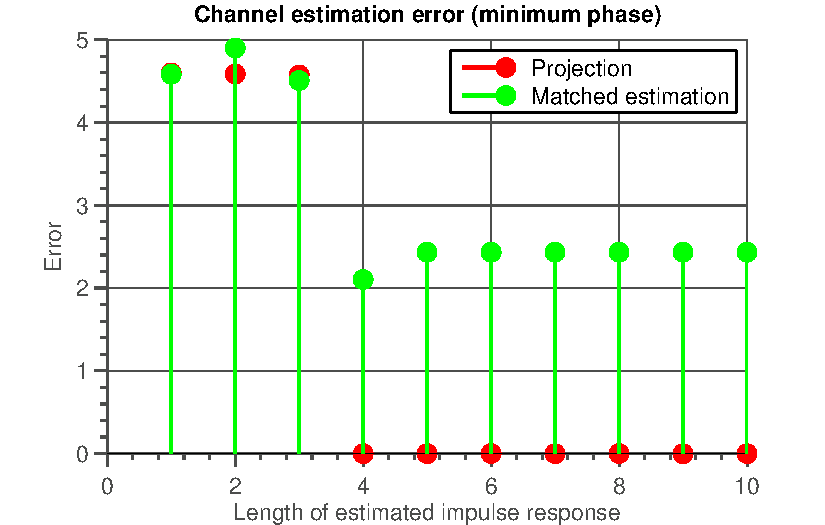
\includegraphics[width=\textwidth]{../../deliverable-7-resources/figures/ass-1/report-8-9-10/report-9-no-noise/ass-1-report-9-minimum-phase.pdf}
		\caption{\centering Channel estimation error for a minimum phase sequence}
	\end{subfigure}
	\begin{subfigure}{0.49\textwidth}
		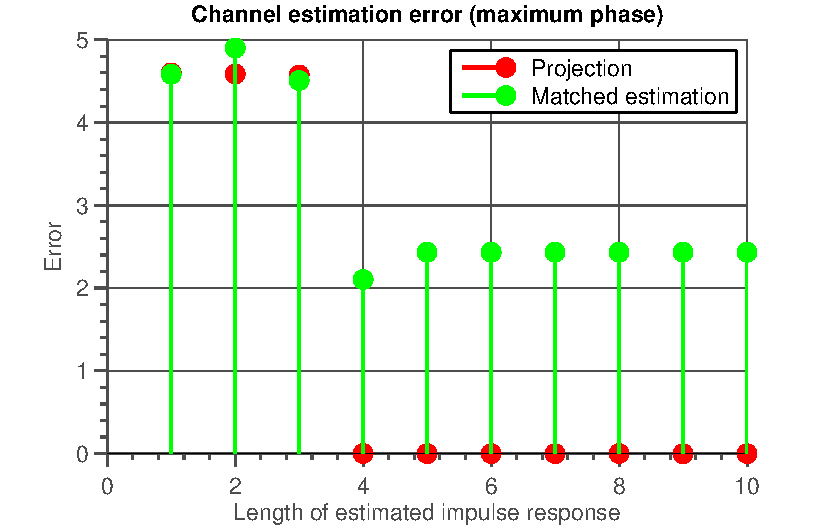
\includegraphics[width=\textwidth]{../../deliverable-7-resources/figures/ass-1/report-8-9-10/report-9-no-noise/ass-1-report-9-maximum-phase.pdf}
		\caption{\centering Channel estimation error for a maximum phase sequence}
	\end{subfigure}
	\begin{subfigure}{0.49\textwidth}
		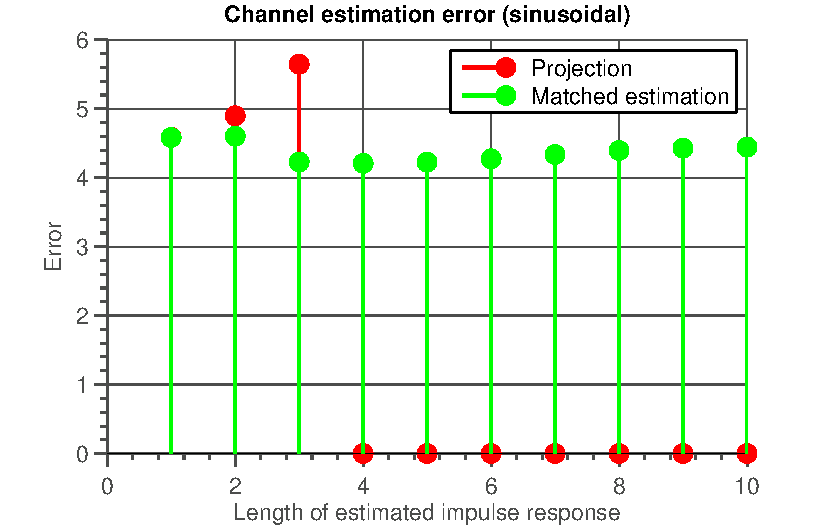
\includegraphics[width=\textwidth]{../../deliverable-7-resources/figures/ass-1/report-8-9-10/report-9-no-noise/ass-1-report-9-sinusoidal.pdf}
		\caption{\centering Channel estimation error for a sinusoidal sequence}
	\end{subfigure}
	\begin{subfigure}{0.49\textwidth}
		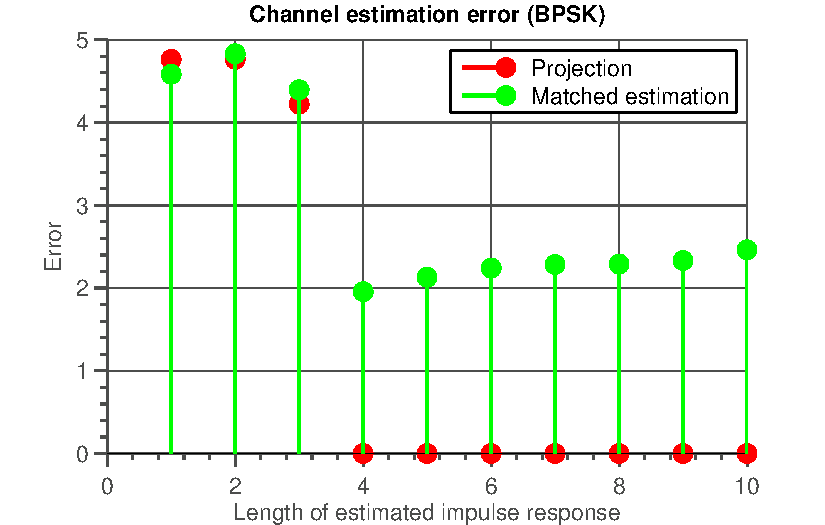
\includegraphics[width=\textwidth]{../../deliverable-7-resources/figures/ass-1/report-8-9-10/report-9-no-noise/ass-1-report-9-BPSK.pdf}
		\caption{\centering Channel estimation error for a BPSK sequence}
	\end{subfigure}
	\caption{The channel estimation error for increasing $\hat{L}$ without noise}
	\label{fig:ass-1-rep-9-no-noise}
\end{figure}

We see that projection, which is deconvolution by calculating the pseudo-inverse, clearly outperforms the matched estimation, which is the estimation by the Matched Filter. Also, projection requires to have $\hat{L} \ge L$ to perform optimally. The matched estimation performs optimally if $\hat{L} = L$. Therefore, we conclude that if $\hat{L}$ is large enough, only the matched estimation is sensitive to the choice of $
\hat{L}$.

Figure~\ref{fig:ass-1-rep-9-0.1} shows the channel estimation error with noise added. The STD $\sigma_{\text{noise}}$ of the noise added is given by $0.1$. We conclude that the conclusions of the previous paragraph still hold. Also, we see that for a large enough $\hat{L}$ the BPSK sequence is the least sensitive to noise. The minimum phase and maximum phase sequences have the least error for the matched estimation.

\begin{figure}[H]
	\centering
	\begin{subfigure}{0.49\textwidth}
		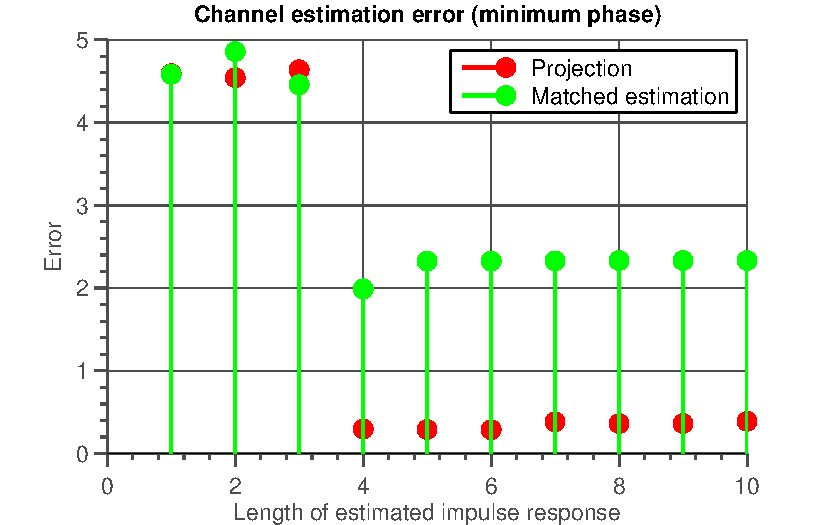
\includegraphics[width=\textwidth]{../../deliverable-7-resources/figures/ass-1/report-8-9-10/report-9-noise-0.1/ass-1-report-9-minimum-phase.pdf}
		\caption{\centering Channel estimation error for a minimum phase sequence}
	\end{subfigure}
	\begin{subfigure}{0.49\textwidth}
		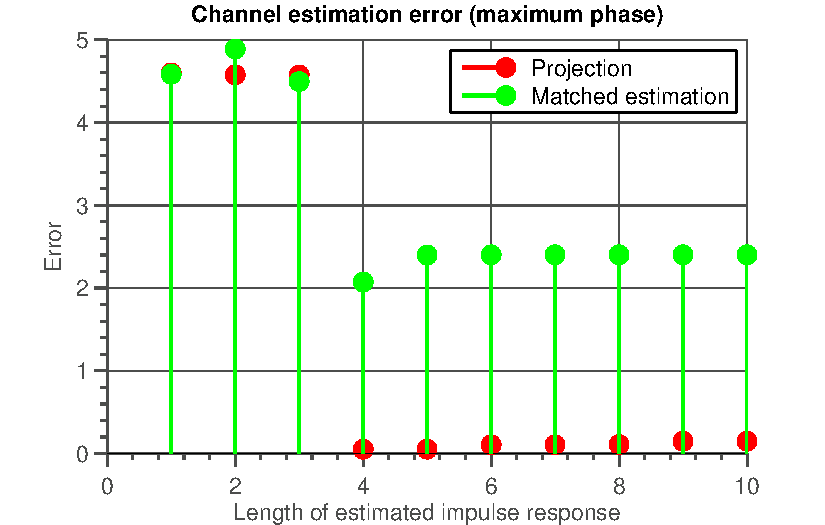
\includegraphics[width=\textwidth]{../../deliverable-7-resources/figures/ass-1/report-8-9-10/report-9-noise-0.1/ass-1-report-9-maximum-phase.pdf}
		\caption{\centering Channel estimation error for a maximum phase sequence}
	\end{subfigure}
	\begin{subfigure}{0.49\textwidth}
		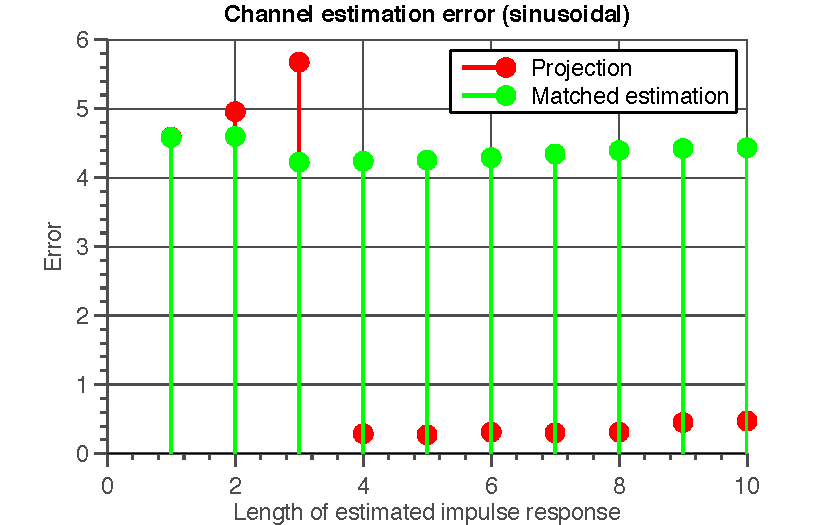
\includegraphics[width=\textwidth]{../../deliverable-7-resources/figures/ass-1/report-8-9-10/report-9-noise-0.1/ass-1-report-9-sinusoidal.pdf}
		\caption{\centering Channel estimation error for a sinusoidal sequence}
	\end{subfigure}
	\begin{subfigure}{0.49\textwidth}
		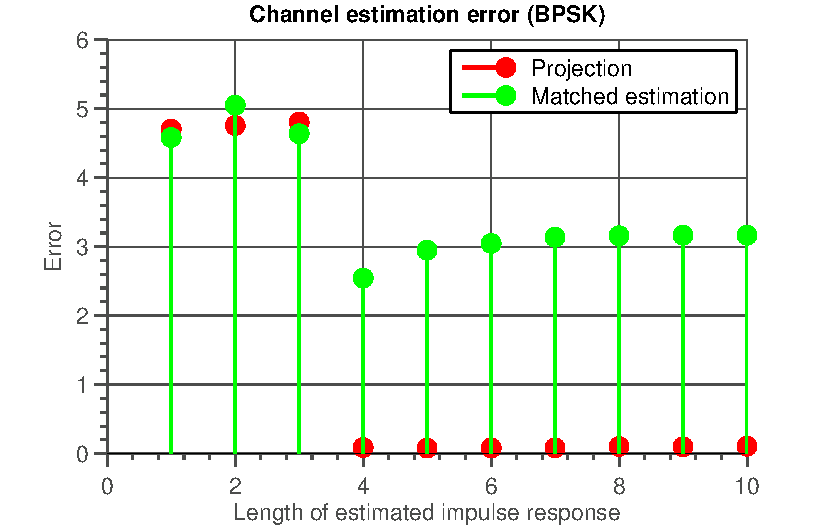
\includegraphics[width=\textwidth]{../../deliverable-7-resources/figures/ass-1/report-8-9-10/report-9-noise-0.1/ass-1-report-9-BPSK.pdf}
		\caption{\centering Channel estimation error for a BPSK sequence}
	\end{subfigure}
	\caption{The channel estimation error for increasing $\hat{L}$, with $\sigma_{\text{noise}} = 0.1$}
	\label{fig:ass-1-rep-9-0.1}
\end{figure}


\subsection{Report 10}
\label{subsec:ass-1-rep-10}
In this report we will discuss three aspects of our training sequence and the channel estimation; \textbf{(1)} the trainings sequence's length $N$, \textbf{(2)}, the estimated impulse response's length $\hat{L}$ and \textbf{(3)}, the properties of the training sequence itself.

The training sequence's length should be chosen in consideration with the properties of the training sequence itself so that \textbf{(a)}, an autocorrelation which resembles a delta function, \textbf{(b)}, a crosscorrelation with every other signal of zero and \textbf{(c)}, a minimal length to minimize computations and maximize speed are achieved. A trade-off has to be made between \textbf{(a)} and \textbf{(c)}, so these are design choices. Also, to satisfy \textbf{(c)}, $\hat{L}$ should be chosen so that it matches the actual channel impulse response's length $L$.
\end{document}